\section{Технический проект}
\subsection{Общая характеристика организации решения задачи}

Необходимо спроектировать и разработать интеллектуальную систему распознавания пятен разливов нефти на поверхности водоемов.

Интеллектуальная система состоит из модели нейронной сети и приложения, отвечающего за взаимодействие пользователей с системой. В приложении необходимо иметь возможность взаимодействовать с нейронной сетью при помощи графического интерфейса пользователя. Под взаимодействием понимается загрузка изображений, содержащих пятна нефтяных разливов, возможность распознавания пятен при помощи модели нейронной сети, а также её обучение и тестирование.

\subsection{Обоснование выбора технологии проектирования}

Технологии, языки программирования и архитектурные решения, использованные для создания интеллектуальной системы, отвечают современным практикам разработки и позволяют достичь высокой производительности и отказоустойчивости программы.

\subsubsection{Язык программирования Python}

Для реализации программной системы был использован язык Python. Python -- язык программирования высокого уровня, обладающий высокой степенью гибкости и широко используемый как в научной отрасли, так и для коммерческой разработки. Особенно хорошо Python подходит для построения интеллектуальных систем и анализа изображений благодаря богатой системе внешних библиотек, позволяющих значительно упростить построение модели нейронной сети, подготовку данных, работу с изображениями, создание графического интерфейса пользователя. 
Интуитивный синтаксис языка позволяет снизить количество синтаксических ошибок, что в свою очередь значительно ускоряет разработку программных продуктов. Встроенная поддержка различных парадигм программирования позволяет удобно реализовывать модульную архитектуру приложения с использованием классов, функций и последовательного кода. Кроссплатформенность языка облегчает адаптацию системы для работы на различных операционных систем, что при желании позволит легко создать нативные версии приложений для таких операционных систем, как Linux и macOS.


\subsubsection{Описание библиотеки PyTorch}
	
Для разработки модели нейронной сети была выбрана библиотека PyTorch. PyTorch является открытой библиотекой, содержащей широкий	набор инструментов для машинного обучения. Данная библиотека активно применяется в разнообразных научных исследованиях, использующих модели нейронных сетей. PyTorch зарекомендовала себя благодаря гибкости, лаконичному синтаксису и обширным возможностям построения и обучения нейронных сетей. 

Для определения структуры вычислений PyTorch использует динамический вычислительный граф, что означает построение графа операций непосредственно в процессе выполнения программы вместо предварительного определения его структуры. Данный подход значительно упрощает модификацию и отладку архитектуры модели нейронной сети, позволяет удобно реализовывать операции обучения, тестирования и анализа при помощи полученной модели нейронной сети. 

\subsubsection{Описание библиотеки OpenCV}

OpenCV -- одна из наиболее часто применяемых библиотек в области компьютерного зрения и обработки изображений. Она позволяет реализовать значительное количество операций для работы с изображениями и видео, таких как фильтрация, преобразования, геометрические операции. Высокая производительность позволяет эффективно читать, изменять размеры и форматы изображений, создавать их маски, визуализировать результаты работы интеллектуальной системы. 

\subsubsection{Описание фреймворка PyQt6}

PyQt6 является набором расширений кросплатформенного графического фреймворка Qt 6 версии для языка Python. PyQt6 позволяет создавать графические интерфейсы пользователя различной сложности -- от простых оконных приложений до многооконных систем с развитой логикой взаимодействий. 

Одним из ключевых преимуществ PyQt6 является большое число готовых элементов графического интерфейса, таких как кнопки, выпадающие списки, таблицы, позволяющих строить полноценный интуитивный пользовательский интерфейс. Графический интерфейс PyQt можно разрабатывать как вручную в коде, так и при помощи визуального редактора Qt Designer, возвращающего пользователю готовый Python-код для графического интерфейса. Кроссплатформенность PyQt6 позволяет запускать приложения, разработанные для операционной системы Windows на компьютерах с Linux и macOS не требуя значительных изменений, что позволяет без особых усилий создавать мультиплатформенные версии приложений.

\subsubsection{Описание библиотеки NumPy}

Библиотека NumPy предназначена для работы с многомерными массивами и матрицами, а также позволяет проводить сложные математические вычисления с высокой скоростью. NumPy предлагает большое количество функций для работы с массивами, таких как арифметические и логические операции, линейная алгебра. 

NumPy позволяет преобразовывать изображения и их маски в числовые массивы для дальнейшей обработки, а также объединять и нормализовать эти маски. Компактный синтаксис и высокая производительность делают его подходящим для практически любых проектов, связанных с обработкой данных. 

\subsection{Архитектура программной системы}

На рисунке~\ref{fig:structure} в виде UML-диаграммы представлена архитектура программной системы.  

\begin{figure}[h]
	\centering
	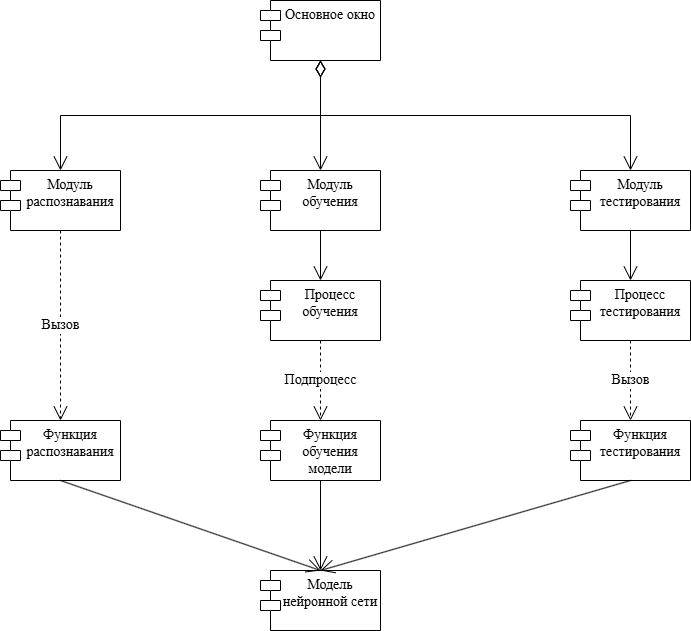
\includegraphics[width=0.85\linewidth]{images/компоненты}
	\caption{Архитектура системы}
	\label{fig:structure}
\end{figure}

Интеллектуальная система состоит из следующих компонентов:
\begin{enumerate}
	\item Основное окно. Основное окно отвечает за вызов главного окна программной системы и инициализацию трех режимов работы программы и переключение между ними.
	\item Модуль распознавания. Данный модуль вызывает окно для распознавания изображения, позволяющее выбрать изображение и параметры модели для анализа нейронной сетью, запускает процесс распознавания и отображает результат.
	\item Функция распознавания. Использует модель нейронной сети и ее параметры для анализа полученного изображения, возвращая результат работы и сохраняя его в виде файла.
	\item Модуль обучения. Вызывает окно, позволяющее выбрать директорию, содержащую изображения для обучения нейронной сети, и указать директорию для сохранения файла параметров обученной нейронной сети. Кроме того, данный модуль запускает процесс, отвечающий за обучение нейронной сети и отображение прогресса завершения обучения. 
	\item Функция обучения модели. Компонент загружает изображения для обучения, преобразует их в требуемый для обучения нейронной сети вид и обучает модель, сохраняя полученный в результате файл параметров.
	\item Модуль тестирования. Вызывает окно, позволяющее выбрать параметры модели, тестовое изображение и запускает процесс, отвечающий за тестирование модели нейронной сети с сохраненными параметрами и возвращает результаты тестирования. Также отображает полученные метрики и результаты.
	\item Функция тестирования. Выполняет оценку точности модели нейронной сети с параметрами, загруженными из предварительно сохраненного файла. Сравнивает результат анализа изображения нейронной сетью и ожидаемый результат, полученный при помощи пороговой фильтрации.
	\item Модель нейронной сети. Хранит в себе структуру используемой в системе нейронной сети. 
\end{enumerate}

\subsection{Выбор структуры нейронной сети}

Для распознавания нефтяных пятен на изображениях поверхностей водоемов была спроектирована и разработана модель сверточной нейронной сети. Сверточные нейронные сети -- однонаправленные модели, разработанные для распознавания образов на изображениях. В данной работе была реализована нейронная сеть типа U-Net, адаптированная под особенности предметной области. 

Архитектура U-Net была представлена в 2015 году группой исследователей из Университета Фрайбугра. Данная архитектура получила широкое распространение благодаря способности выделять объекты различной формы и масштаба с высокой точностью даже на маленьких обучающих выборках. Основной особенностью U-Net является симметричная структура: левая часть сети, или энкодер, выполняет последовательное сжатие входного изображения, а правая, или декодер -- восстановление пространственного разрешения до исходного размера.

\begin{figure}[h]
	\centering
	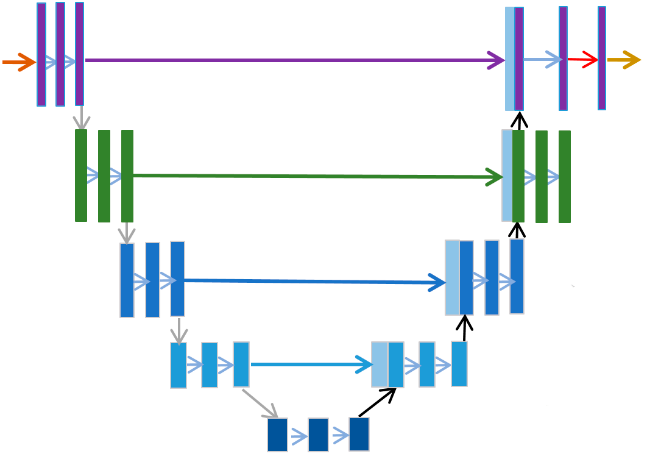
\includegraphics[width=0.85\linewidth]{images/unet}
	\caption{Архитектура сети U-Net}
	\label{fig:unet}
\end{figure}

Ключевым элементом U-Net являются прямые соединения между соответствующими уровнями энкодера и декодера, позволяющие использовать признаки, извлеченные на ранних этапах обработки, передавая их на этапы восстановления изображения, что предотвращает потерю пространственной информации. Данные особенности позволяют с легкостью адаптировать U-Net для использования в различных областях, например медицинская диагностика, спутниковый мониториг, обработка изображений, полученных с беспилотных летательных аппаратов.

\subsection{Проектирование пользовательского интерфейса}

На основании требований к пользовательскому интерфейсу, представленных в пункте 2.3.3, был разработан графический интерфейс программной системы. 

На рисунке~\ref{fig:uianalysis} представлен макет интерфейса окна "<Анализ изображения">. Макет содержит следующие элементы:

\begin{enumerate}
	\item Кнопка переключения режимов окна.
	\item Поле, содержащее путь до анализируемого изображения.
	\item Кнопка выбора изображения для анализа.
	\item Поле, содержащее путь до выбранного файла параметров нейронной сети.
	\item Кнопка выбора файла параметров нейронной сети.
	\item Поле для отображения загруженного изображения и результатов анализа.
	\item Кнопка для запуска распознавания нефтяных пятен. 
	\item Кнопка для сохранения результатов анализа нейронной сети.
\end{enumerate}

\begin{figure}[H]
	\centering
	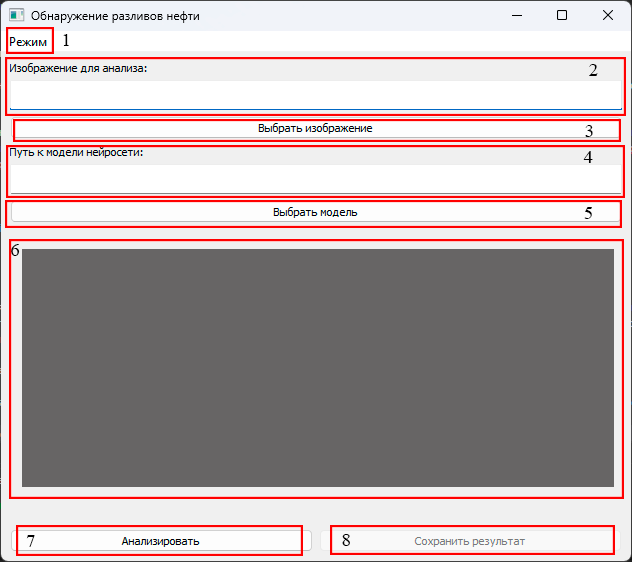
\includegraphics[width=1\linewidth]{images/ui_analysis}
	\caption{Макет интерфейса окна «Анализ изображения»}
	\label{fig:uianalysis}
\end{figure}

На рисунке~\ref{fig:uitrain} представлен макет интерфейса окна "<Обучение">. Макет содержит следующие элементы:

\begin{enumerate}
	\item Кнопка переключения режимов окна.
	\item Поле, содержащее путь до выбранной папки с изображениями для обучения нейронной сети.
	\item Кнопка выбора папки с изображениями для обучения нейронной сети.
	\item Поле, содержащее путь до папки, в которую необходимо сохранить параметры модели.
	\item Кнопка для выбора папки, в которую необходимо сохранить параметры модели.
	\item Окно для вывода прогресса обучения нейронной сети.
	\item Кнопка для запуска процесса обучения нейронной системы.
\end{enumerate}

\begin{figure}[H]
	\centering
	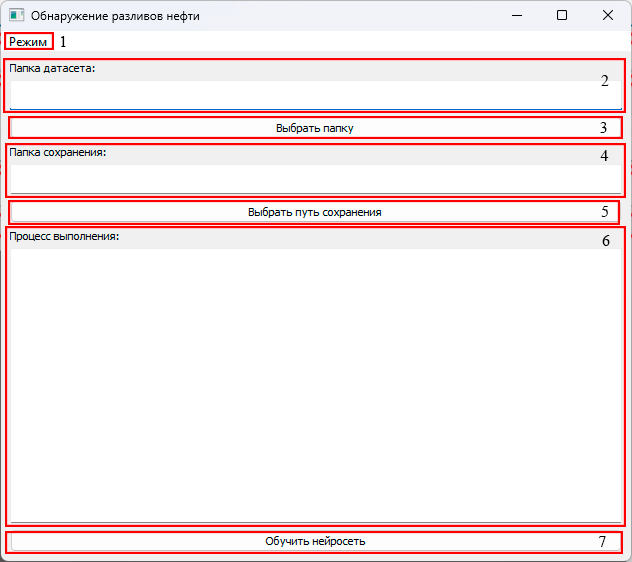
\includegraphics[width=1\linewidth]{images/ui_train}
	\caption{Макет интерфейса окна «Обучение»}
	\label{fig:uitrain}
\end{figure}

На рисунке~\ref{fig:uitest} представлен макет интерфейса окна "<Тестирование">. Макет содержит следующие элементы:

\begin{enumerate}
	\item Кнопка переключения режимов окна.
	\item Поле, содержащее путь до тестового изображения.
	\item Кнопка выбора изображения для тестирования нейронной сети.
	\item Поле, содержащее путь до выбранного файла параметров нейронной сети.
	\item Кнопка выбора файла параметров нейронной сети.
	\item Поле вывода метрик тестирования нейронной сети.
	\item Поле для отображения исходного изображения.
	\item Поле для отображения ожидаемого результата обработки.
	\item Поле для отображения фактического результата обработки изображения нейронной сети.
	\item Кнопка для запуска тестирования.
\end{enumerate}

\begin{figure}[H]
	\centering
	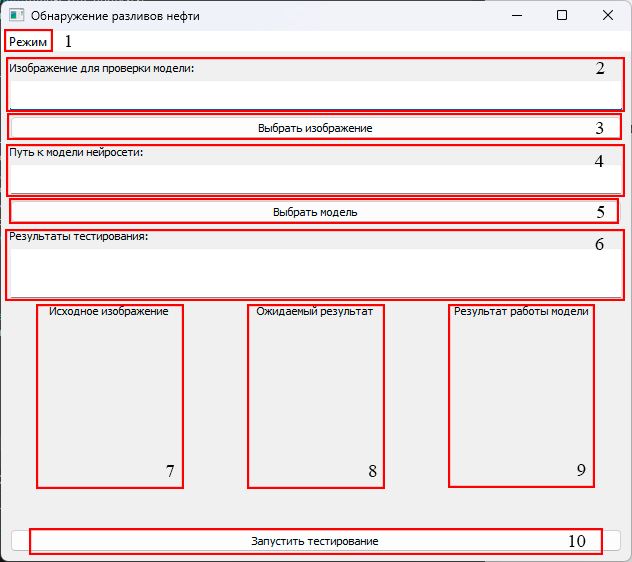
\includegraphics[width=1\linewidth]{images/ui_test}
	\caption{Макет интерфейса окна «Тестирование»}
	\label{fig:uitest}
\end{figure}

\newpage